\documentclass{beamer}
\usepackage[utf8]{inputenc}

\author[Sowmya Vajjala]{Instructor: Sowmya Vajjala}


\title[LING 120]{LING 120, Fall 2017: \\ Language and Computers}
\subtitle{Topic: Overview of Natural Language Processing}

\date{13 October 2017 (Week 8)}

\institute{Iowa State University, USA}

\usepackage{graphicx}
%%%%%%%%%%%%%%%%%%%%%%%%%%%

\begin{document}

\begin{frame}\titlepage
\end{frame}

\begin{frame}%2minutes
\frametitle{Class outline}
\begin{itemize}
\item Midterms: comments
\item Assignment 3 discussion
\item General Review and discussion of topics
\item Feedback on the course so far.
\end{itemize}
\end{frame}

\begin{frame}
\frametitle{Midterms: Comments}
\begin{itemize}
\item 6 teams: voice recognition (1), duo lingo (3), regular expressions (2)
\item Good show - perfect scores! (to be fair, I also did not nitpick!)
\item Content: Lot of new stuff beyond what was discussed in the class. Hopefully, all of you enjoyed as much as I did! 
\item presentation issues: maintaining co-ordination between presenters, eye-contact with audience, taking care about what is put on slides, sticking to time etc. (those can improve with practice and experience!)
\end{itemize}
\end{frame}

\begin{frame}
\frametitle{Voice Recognition}
\begin{itemize}
\item Loved those spectrogram images! 
\item Good observations about Dictation tool.
\item Wishlist: someone doing this for multiple languages and comparing accuracy of speech recognition for some non-English language (with accents!)
\end{itemize}
\end{frame}

\begin{frame}
\frametitle{Duolingo presentations}
 \begin{itemize}
 \item Duo Lingo - different languages, exercise sequences, advanced level exercises, writing systems, comparison with classroom learning, grammar
\item languages discussed: English, German, Greek, Chinese, Hebrew, Italian, Japanese, Russian, Spanish, Ukranian
\item Hopefully, you learnt more about tutoring systems than what is in the textbook!
\end{itemize}
\end{frame}

\begin{frame}
\frametitle{Regular Expressions Presentations}
 \begin{itemize}
 \item Searching through code, searching in MS Word with Macros.
\item Nice examples/videos/demos.
\item A little bit of complex stuff for non-CS people, something you could work on in terms communicating to a broader audience.
 \end{itemize}
\end{frame}

\begin{frame}
\frametitle{Assignment 3 discussion}
 \begin{itemize}
 \item 1 (a): Duolingo vs TAGARELA
\item 1 (b):  British council test - not adaptive (most of you - perhaps the ones who tried it twice) got it right. 	
\item 2 (a): "he", "assembly", 3170. Most diverse answers are here :-) 
\item 2 (b): Amazon vs the search engine X. 
 \end{itemize}
\end{frame}

\begin{frame}
\frametitle{General Remarks}
 \begin{itemize}
\item When you don't understand something, ask.
\item Office hours: Monday, Wednesday 1--2 pm. Ross 331 \pause
\item If you don't tell me, I cannot know you are having difficulties.
\item Participate in the class, or online, or talk to me in person if you are too shy. \pause
\item It is just another course, yes, but why lose grade in a 100-level course unnecessarily?
 \end{itemize}
\end{frame}

\begin{frame}
\frametitle{General Review of Topics so far}
We finished half of the book (and more!!!)
\begin{enumerate}
\item Encoding and inputting text and speech on computers
\item Writers aids - the only topic which no one chose for midterms :-)
\item Language tutoring systems
\item Searching
\item Overview of natural language processing
\end{enumerate}
(3 assignments and 1 mid-term done!)
\end{frame}

\begin{frame}
\frametitle{Whats in store next?}
\begin{enumerate}
\item Quick overview of language and cryptography 
\item automatically classifying text (e.g., spam email classification)
\item Dialog systems, speech based human-machine interaction
\item Machine translation
\end{enumerate}
\end{frame}

\begin{frame}%2minutes
\frametitle{Next week}
\begin{itemize}
\item Topic: (mainly) Text classification
\item Readings: Chapter 5 in the textbook
\item Deadlines: Assignment 4 (21st October)
\end{itemize}
\end{frame}

\begin{frame}%2minutes
\frametitle{What is text classification?}
\framesubtitle{A randomly picked student should answer each question!}
\begin{itemize}
\item if I say spam email classification as an example, what are some other such practical applications you can think of? \pause
\item How easy is it to do spam classification for humans? \pause 
\\ Is this spam?
\\ 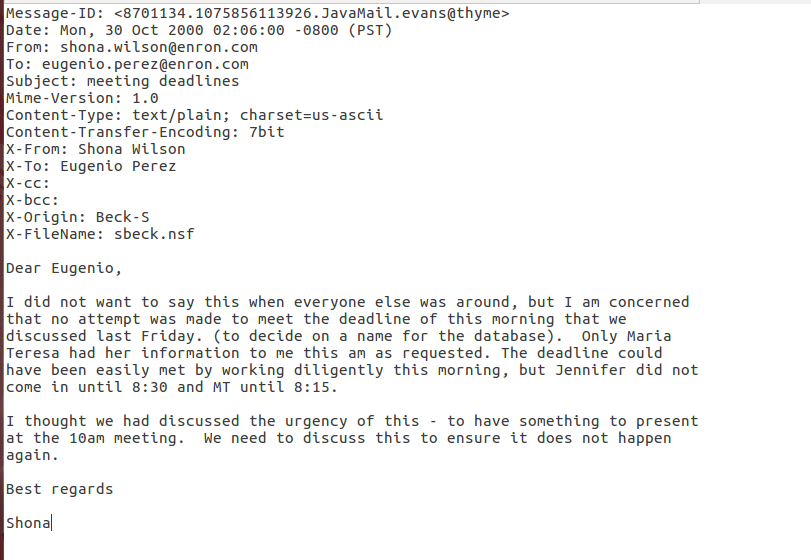
\includegraphics[width=0.9\textwidth]{ham.png}
\end{itemize}
\end{frame}

\begin{frame}%2minutes
\frametitle{Is this spam?}
\framesubtitle{Source for both these pics: Enron spam dataset}
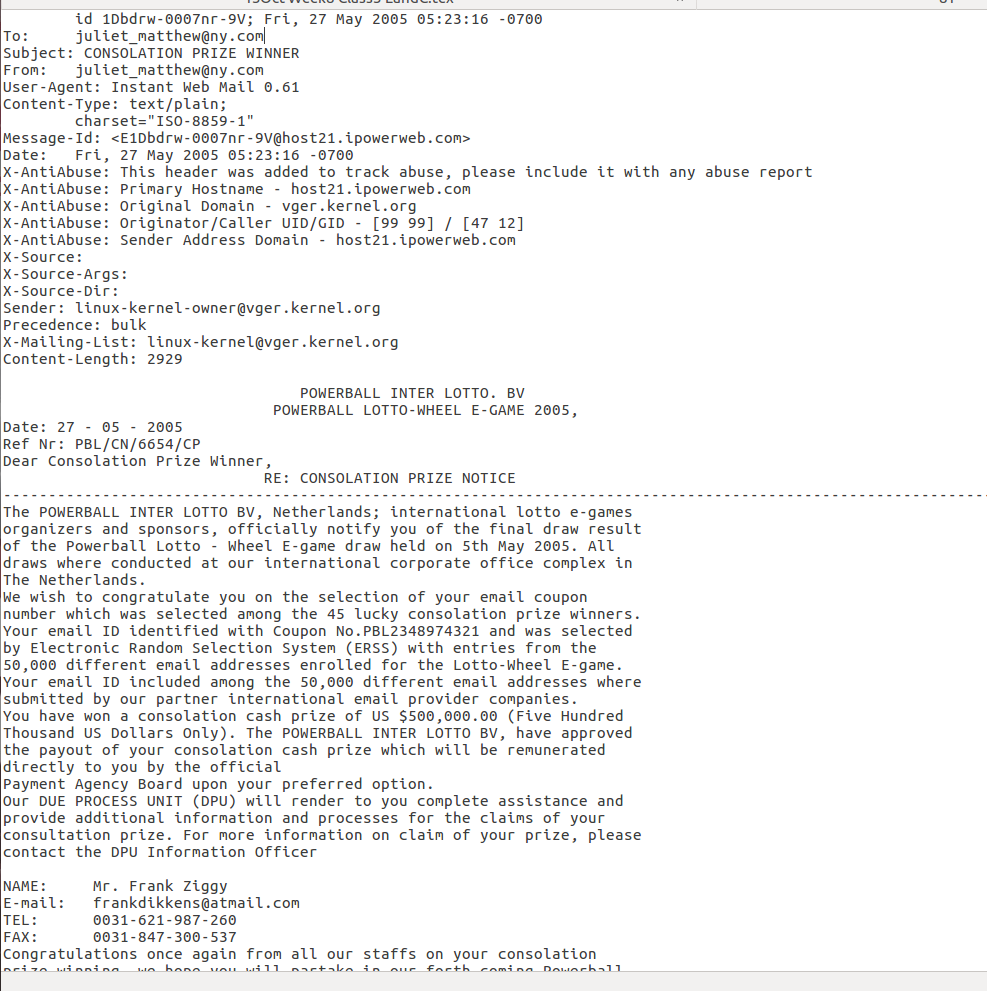
\includegraphics[width=0.9\textwidth]{spam.png}
\\ \url{http://www.aueb.gr/users/ion/data/enron-spam/}
\end{frame}

\begin{frame}%2minutes
\frametitle{Spam in SMS: What is spam?}
\begin{itemize}
\item "Did you catch the bus ? Are you frying an egg ? Did you make a tea? Are you eating your mom's left over dinner ? Do you feel my Love ?"
\item "Forwarded from 44871240400: Please CALL 08712404000 immediately as there is an urgent message waiting for you."
\item "Do you realize that in about 40 years, we'll have thousands of old ladies running around with tattoos?"
\item "Realy sorry-i don't recognise this number and am now confused :) who r u please?! "
\end{itemize}
source: online spam dataset. \url{https://goo.gl/7Dq85S}
\end{frame}

\begin{frame}%2minutes
\frametitle{Spam vs Ham - is it so easy?}
\begin{itemize}
\item Not always. A job ad is perhaps not spam. But if the same ad comes repeatedly, it is.
\item A group email is not a spam for someone. But it is, for others.
\item Is it easier or difficult with SMS compared to email? \pause
\item Are you satisfied with your email provider's spam classification? \pause
\item What do you think it is doing? 
\end{itemize}
\end{frame}


\begin{frame}
\frametitle{Feedback about the course}
\begin{itemize}
\item Please fill up the form given (all the 4 blocks)
\item whats in it for you: you can see some improvements for the rest of the semester
\item whats in it for me: feedback to improve teaching practices
\item whats in it for future students: a better designed course
\end{itemize}
\end{frame}

\end{document}
